% =============================================================================
%  PINN Literature Review — Presentation Slides
%  Author: G. Scriven (LHCb, Nikhef)
%  Date:   March 2026
% =============================================================================
\documentclass[aspectratio=169, 11pt]{beamer}

% ---- Theme & Colours --------------------------------------------------------
\usetheme{Madrid}
\usecolortheme{default}

\definecolor{lhcbblue}{HTML}{1F77B4}
\definecolor{nngreen}{HTML}{2CA02C}
\definecolor{rkorange}{HTML}{FF7F0E}
\definecolor{rk4red}{HTML}{D62728}
\definecolor{lightgray}{HTML}{F0F0F0}
\definecolor{darkgray}{HTML}{404040}

\setbeamercolor{title}{fg=white, bg=lhcbblue}
\setbeamercolor{frametitle}{fg=white, bg=lhcbblue}
\setbeamercolor{structure}{fg=lhcbblue}
\setbeamercolor{block title}{bg=lhcbblue!20, fg=black}
\setbeamercolor{block body}{bg=lhcbblue!5}
\setbeamercolor{block title alerted}{bg=rk4red!20, fg=black}
\setbeamercolor{block body alerted}{bg=rk4red!5}
\setbeamercolor{block title example}{bg=nngreen!20, fg=black}
\setbeamercolor{block body example}{bg=nngreen!5}
\setbeamertemplate{navigation symbols}{}
\setbeamertemplate{footline}[frame number]

% ---- Packages ---------------------------------------------------------------
\usepackage[utf8]{inputenc}
\usepackage[T1]{fontenc}
\usepackage{lmodern}
\usepackage{amsmath,amssymb}
\usepackage{booktabs}
\usepackage{array}
\usepackage{colortbl}
\usepackage{xcolor}
\usepackage{tikz}
\usetikzlibrary{arrows.meta, positioning, shapes.geometric, calc, fit}
\usepackage{hyperref}
\usepackage{bm}
\newcommand{\vb}[1]{\bm{#1}}

% =============================================================================
\title[PINN Literature Review]{%
  \textbf{Physics-Informed Neural Networks}\\[4pt]
  \large Literature Review for Track Extrapolation}

\author{G.~Scriven}
\institute{Maastricht University\quad$\cdot$\quad UHasselt\quad$\cdot$\quad LHCb}
\date{March 2026}

\begin{document}

% =============================================================================
% TITLE SLIDE
% =============================================================================
\begin{frame}[plain]
  \titlepage
\end{frame}

% =============================================================================
% OUTLINE
% =============================================================================
\begin{frame}{Outline}
  \tableofcontents
\end{frame}

% =============================================================================
\section{Motivation}
% =============================================================================

\begin{frame}{The Track Extrapolation Problem}
  \begin{columns}[T]
    \column{0.55\textwidth}
    \textbf{Goal:} Replace C++ RK4 track extrapolator with a neural network.

    \medskip
    Lorentz force ODEs:
    \begin{align*}
      \frac{dt_x}{dz} &= \kappa N \bigl[ t_x t_y B_x - (1{+}t_x^2) B_y + t_y B_z \bigr] \\
      \frac{dt_y}{dz} &= \kappa N \bigl[ (1{+}t_y^2) B_x - t_x t_y B_y - t_x B_z \bigr]
    \end{align*}
    where $\kappa = (q/p)\cdot c_\text{light}$, $N = \sqrt{1+t_x^2+t_y^2}$.

    \medskip
    Learn the mapping:
    \[
      f_\theta: (x_0, y_0, t_{x,0}, t_{y,0}, q/p, \Delta z) \to (x_f, y_f, t_{x,f}, t_{y,f})
    \]

    \column{0.42\textwidth}
    \begin{block}{V1 Key Results}
      \centering\small
      \begin{tabular}{lrr}
        \toprule
        \textbf{Model} & \textbf{$\mu$s} & \textbf{Error} \\
        \midrule
        MLP tiny    & 1.12 & 53\,$\mu$m \\
        MLP medium  & 2.17 & 37\,$\mu$m \\
        PINN        & 2.46 & \textcolor{rk4red}{593\,mm} \\
        RK-PINN     & 5.59 & \textcolor{rk4red}{2\,km} \\
        \midrule
        C++ RK4     & 2.50 & 0 (ref.) \\
        \bottomrule
      \end{tabular}
    \end{block}

    \begin{alertblock}{PINNs failed!}
      Errors $10^4\times$ worse than MLPs. \\
      \textbf{Root cause:} IC violation bug.
    \end{alertblock}
  \end{columns}
\end{frame}

% -----------------------------------------------------------------------------
\begin{frame}{Why PINNs Failed in V1}
  \begin{columns}[T]
    \column{0.48\textwidth}
    \textbf{The bug:} \texttt{forward()} hardcoded $z_\text{frac}=1.0$
    \begin{itemize}
      \item Network never saw intermediate trajectory points
      \item Physics loss at collocation points evaluated \emph{untrained} regime
      \item Output independent of $z$ $\Rightarrow$ IC violated
    \end{itemize}

    \medskip
    \textbf{Additional issues:}
    \begin{itemize}
      \item Gaussian field approximation $\neq$ real field map
      \item Only weak $t_y$ conservation constraint
      \item 50M samples made data loss dominant
    \end{itemize}

    \column{0.48\textwidth}
    \begin{exampleblock}{Proposed Fix: PINN\_v3}
      Residual architecture guarantees IC:
      \[
        \vb{y}(z) = \vb{y}_0 + z_\text{frac} \cdot \text{MLP}(\vb{y}_0, q/p, \Delta z)
      \]
      \begin{itemize}
        \item At $z_\text{frac}=0$: $\vb{y}(0) = \vb{y}_0$ \checkmark
        \item Smooth interpolation guaranteed
        \item Not yet trained in V1
      \end{itemize}
    \end{exampleblock}
  \end{columns}

  \bigskip
  \centering
  \textcolor{lhcbblue}{\textbf{Question:} What does the literature say about these issues?}
\end{frame}

% =============================================================================
\section{Original PINN Papers}
% =============================================================================

\begin{frame}{The PINN Framework}
  \textbf{Raissi, Perdikaris \& Karniadakis} (2019) --- \textit{J.\ Comput.\ Phys.}

  \begin{columns}[T]
    \column{0.55\textwidth}
    \begin{itemize}
      \item Neural network $u_\theta(x,t)$ approximates PDE solution
      \item Physics residual added to loss function:
        \[
          \mathcal{L} = \underbrace{\mathcal{L}_\text{data}}_{\text{boundary/IC}} + \lambda \underbrace{\mathcal{L}_\text{PDE}}_{\text{residual at collocation pts}}
        \]
      \item Derivatives computed via automatic differentiation
      \item Demonstrated on Burgers', Schr\"odinger, Navier--Stokes
      \item \textbf{Foundational paper} --- 10,000+ citations
    \end{itemize}

    \column{0.42\textwidth}
    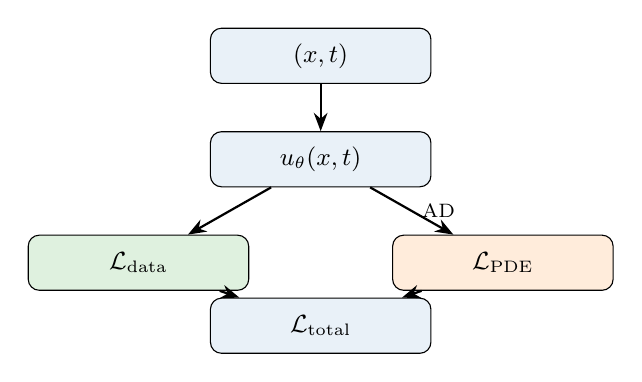
\begin{tikzpicture}[
      box/.style={draw, rounded corners, fill=lhcbblue!10, minimum width=2.8cm, minimum height=0.7cm, align=center, font=\small},
      arrow/.style={-Stealth, thick}
    ]
      \node[box] (input) {$(x, t)$};
      \node[box, below=0.6cm of input] (nn) {$u_\theta(x,t)$};
      \node[box, below left=0.6cm and -0.5cm of nn, fill=nngreen!15] (data) {$\mathcal{L}_\text{data}$};
      \node[box, below right=0.6cm and -0.5cm of nn, fill=rkorange!15] (pde) {$\mathcal{L}_\text{PDE}$};
      \node[box, below=0.8cm of nn, yshift=-0.6cm] (loss) {$\mathcal{L}_\text{total}$};

      \draw[arrow] (input) -- (nn);
      \draw[arrow] (nn) -- (data);
      \draw[arrow] (nn) -- node[right, font=\scriptsize] {AD} (pde);
      \draw[arrow] (data) -- (loss);
      \draw[arrow] (pde) -- (loss);
    \end{tikzpicture}
  \end{columns}
\end{frame}

% =============================================================================
\section{Paper 1: FD-PINN}
% =============================================================================

\begin{frame}{Paper 1: Finite Difference PINNs}
  \textit{``Physics-informed deep learning based on the finite difference method for efficient and accurate numerical solution of PDEs''}

  \begin{columns}[T]
    \column{0.55\textwidth}
    \textbf{Core idea:} Replace automatic differentiation with finite differences.
    \[
      \frac{\partial \hat{u}}{\partial x}\bigg|_{x_i} \approx \frac{\hat{u}(x_i + \delta) - \hat{u}(x_i - \delta)}{2\delta}
    \]

    \textbf{Advantages:}
    \begin{itemize}
      \item No computational graph storage $\Rightarrow$ lower memory
      \item Faster training (FD $\approx$ forward passes only)
      \item Works with \textbf{non-differentiable} components
      \item Tested on Burgers', convection--diffusion, Navier--Stokes
    \end{itemize}

    \column{0.42\textwidth}
    \begin{alertblock}{Direct relevance to V1}
      V1 was \textbf{forced} to use a Gaussian field model because AD requires differentiability:
      \[
        B_y(z) = B_0\, e^{-(z-z_c)^2/2\sigma_z^2}
      \]
      With FD, the tabulated field map (\texttt{twodip.rtf}) can be used \textbf{directly}.
    \end{alertblock}

    \begin{exampleblock}{Impact}
      Eliminates the field model mismatch --- the dominant V1 physics loss issue.
    \end{exampleblock}
  \end{columns}
\end{frame}

% =============================================================================
\section{Paper 2: Data-Free PINNs}
% =============================================================================

\begin{frame}{Paper 2: Learning Without Data}
  \textit{Misyris, Stiasny \& Chatzivasileiadis} --- \textit{IEEE SmartGridComm} (2021)

  \begin{columns}[T]
    \column{0.55\textwidth}
    \textbf{Core idea:} Train PINNs with \emph{zero} training data.
    \[
      \mathcal{L} = \lambda_\text{PDE}\,\mathcal{L}_\text{PDE} + \lambda_\text{IC}\,\mathcal{L}_\text{IC} + \lambda_\text{BC}\,\mathcal{L}_\text{BC}
    \]

    \textbf{Key results:}
    \begin{itemize}
      \item Solved DAEs for power grid simulation
      \item Orders-of-magnitude speedup over numerical solvers
      \item Single network solves families of ICs
      \item No data generation infrastructure needed
    \end{itemize}

    \column{0.42\textwidth}
    \begin{block}{Comparison with V1}
      \centering\small
      \begin{tabular}{lcc}
        \toprule
        & \textbf{V1} & \textbf{Paper 2} \\
        \midrule
        Data & 50M & \textbf{0} \\
        Input dim & 6D & 1--3D \\
        Loss & data+PDE & PDE only \\
        \bottomrule
      \end{tabular}
    \end{block}

    \begin{exampleblock}{Implication}
      Pure data-free unlikely for 6D LHCb problem. \\
      \textbf{Hybrid:} 1--5M samples + physics loss for regularisation.
    \end{exampleblock}
  \end{columns}
\end{frame}

% =============================================================================
\section{Paper 3: DeepONet Domain Decomposition}
% =============================================================================

\begin{frame}{Paper 3: Long-Time Integration with DeepONets}
  \textit{``Long-time integration of parametric evolution equations with physics-informed DeepONets''}

  \begin{columns}[T]
    \column{0.55\textwidth}
    \textbf{Problem:} PINNs fail for long integration horizons (spectral bias).

    \textbf{Solution:} \textbf{DeepONet} + temporal domain decomposition.
    \begin{itemize}
      \item DeepONet learns the \emph{solution operator} $\mathcal{G}: u_0 \mapsto u(t)$
      \item Branch net encodes input function; trunk net encodes output locations
      \item Time domain split into short windows; predictions chained
      \item Handles parametric families of ICs
    \end{itemize}

    \column{0.42\textwidth}
    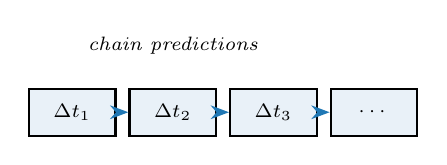
\begin{tikzpicture}[
      win/.style={draw, thick, fill=lhcbblue!10, minimum width=1.1cm, minimum height=0.6cm, font=\scriptsize},
      arrow/.style={-Stealth, thick, lhcbblue}
    ]
      \node[win] (w1) {$\Delta t_1$};
      \node[win, right=0.15cm of w1] (w2) {$\Delta t_2$};
      \node[win, right=0.15cm of w2] (w3) {$\Delta t_3$};
      \node[win, right=0.15cm of w3] (w4) {$\cdots$};
      \draw[arrow] (w1) -- (w2);
      \draw[arrow] (w2) -- (w3);
      \draw[arrow] (w3) -- (w4);
      \node[above=0.3cm of w2, font=\scriptsize\itshape] {chain predictions};
    \end{tikzpicture}

    \medskip
    \begin{alertblock}{Direct relevance to V1}
      V1 fixed $\Delta z = 8000$\,mm. Could not generalise to variable step sizes. \\[2pt]
      \textbf{Chaining short steps} solves this naturally.
    \end{alertblock}
  \end{columns}
\end{frame}

% =============================================================================
\section{Paper 4: RK-PINN}
% =============================================================================

\begin{frame}{Paper 4: Runge--Kutta Structured PINNs}
  \textit{``Parameter estimation and modeling of nonlinear dynamical systems based on RK-PINN''}

  \begin{columns}[T]
    \column{0.55\textwidth}
    \textbf{Core idea:} Embed RK integration structure into the network.
    \[
      \hat{\vb{s}}_\text{out} = \vb{s}_\text{in} + \sum_{k=1}^{4} w_k\,\Delta\vb{s}_k
    \]
    \begin{itemize}
      \item Each stage predicts derivative at intermediate point
      \item Weights initialised to RK4 Butcher tableau
      \item Strong inductive bias $\Rightarrow$ respects ODE structure
      \item Dual: forward simulation + inverse parameter estimation
    \end{itemize}

    \column{0.42\textwidth}
    \begin{block}{V1 RK-PINN vs.\ Literature}
      \centering\small
      \begin{tabular}{lcc}
        \toprule
        & \textbf{V1} & \textbf{Paper 4} \\
        \midrule
        IC guarantee & \textcolor{rk4red}{\textbf{No}} & \textcolor{nngreen}{\textbf{Yes}} \\
        Physics loss & $t_y$ only & Full PDE \\
        Accuracy & 2\,km & Accurate \\
        Inverse & No & Yes \\
        \bottomrule
      \end{tabular}
    \end{block}

    \begin{exampleblock}{Inverse capability}
      Could estimate $q/p$ from track hits $\Rightarrow$ unify extrapolation \& fitting.
    \end{exampleblock}
  \end{columns}
\end{frame}

% =============================================================================
\section{Additional Literature}
% =============================================================================

\begin{frame}{PINN Failure Modes}
  \textbf{Krishnapriyan, Gholami, Zhe, Kirby \& Mahoney} --- \textit{NeurIPS} (2021)

  \textit{``Characterizing possible failure modes in physics-informed neural networks''}

  \begin{columns}[T]
    \column{0.55\textwidth}
    \begin{itemize}
      \item PINNs fail on even \emph{slightly} complex problems
      \item Soft PDE regularisation makes loss landscape ill-conditioned
      \item Failure is \textbf{not} due to limited expressivity --- it's \textbf{optimisation}
      \item Tested: convection, reaction, diffusion operators
    \end{itemize}

    \textbf{Two proposed solutions:}
    \begin{enumerate}
      \item \textbf{Curriculum regularisation:} start simple, increase complexity
      \item \textbf{Sequence-to-sequence:} predict windows, not full space-time
    \end{enumerate}

    \column{0.42\textwidth}
    \begin{alertblock}{Explains V1 failure}
      V1's coupled 4-ODE system with non-uniform field is exactly the ``complex enough to fail'' regime.

      \medskip
      \textbf{Curriculum warmup} was used in V1 (10 epochs) --- but insufficient without the IC fix.
    \end{alertblock}

    \begin{exampleblock}{Remedy}
      Sequence-to-sequence $\equiv$ domain decomposition (Paper~3).
    \end{exampleblock}
  \end{columns}
\end{frame}

% -----------------------------------------------------------------------------
\begin{frame}{Neural Operators: DeepONet \& FNO}
  \begin{columns}[T]
    \column{0.48\textwidth}
    \begin{block}{DeepONet \small (Lu, Jin \& Karniadakis, 2019)}
      \begin{itemize}
        \item Learns \textbf{operators} between function spaces
        \item Branch net: encodes input function at sensors
        \item Trunk net: encodes output locations
        \item High-order error convergence (up to $4^\text{th}$ order)
        \item Published in \textit{Nature Machine Intelligence} (2021)
      \end{itemize}

      \medskip
      \textcolor{lhcbblue}{\textbf{Relevance:}} Could learn $\mathcal{G}: \vb{s}_0 \mapsto \vb{s}(z)$ for \emph{all} initial states \& momenta at once.
    \end{block}

    \column{0.48\textwidth}
    \begin{block}{FNO \small (Li et al., 2020)}
      \begin{itemize}
        \item Parameterises integral kernel in Fourier space
        \item Up to $1000\times$ faster than PDE solvers
        \item Zero-shot super-resolution
        \item Tested: Burgers', Darcy flow, Navier--Stokes
        \item Published at \textit{ICLR} (2021)
      \end{itemize}

      \medskip
      \textcolor{lhcbblue}{\textbf{Relevance:}} Alternative operator architecture. Works best for PDE fields on grids --- less natural for ODE trajectories.
    \end{block}
  \end{columns}

  \medskip
  \centering
  Lu et al.\ (2022, \textit{CMAME}): DeepONet more robust to noise than FNO on 16 benchmarks.
\end{frame}

% =============================================================================
\section{Synthesis \& Roadmap}
% =============================================================================

\begin{frame}{V1 Failures $\leftrightarrow$ Literature Solutions}
  \centering
  \begin{tabular}{p{4.5cm}lp{5cm}}
    \toprule
    \textbf{V1 Failure Mode} & \textbf{Paper} & \textbf{Proposed Solution} \\
    \midrule
    IC violation (PINN ignores $z$) & 2, 4, Failure modes & Residual architecture (PINN\_v3) \\[3pt]
    Field model mismatch & 1 & FD-based physics loss \\[3pt]
    Fixed $\Delta z$ only & 3 & Temporal domain decomposition \\[3pt]
    Weak physics constraint & 4 & Full PDE residual at each stage \\[3pt]
    50M samples required & 2 & Hybrid: few-M data + physics \\[3pt]
    No inverse capability & 4 & Dual forward/inverse RK-PINN \\
    \bottomrule
  \end{tabular}
\end{frame}

% -----------------------------------------------------------------------------
\begin{frame}{Priority Roadmap for V2+}
  \begin{enumerate}
    \item[\textcolor{rk4red}{\textbf{P1}}] \textbf{Fix \& retrain PINN\_v3 + RK-PINN\_v3}
      \begin{itemize}
        \item Residual architecture: $\vb{y}(z) = \vb{y}_0 + z_\text{frac} \cdot \text{MLP}(\cdots)$
        \item \textbf{Prerequisite} for all other improvements
      \end{itemize}

    \medskip
    \item[\textcolor{rkorange}{\textbf{P2}}] \textbf{Adopt FD-based physics loss} (Paper~1)
      \begin{itemize}
        \item Use production field map directly --- no more Gaussian approximation
        \item Low implementation effort; immediate impact
      \end{itemize}

    \medskip
    \item[\textcolor{lhcbblue}{\textbf{P3}}] \textbf{Short-step chaining} (Paper~3)
      \begin{itemize}
        \item Train accurate $\Delta z = 500$--$1000$\,mm model
        \item Chain $N$ steps for longer extrapolations
        \item Compatible with Kalman filter's sequential structure
      \end{itemize}

    \medskip
    \item[\textcolor{nngreen}{\textbf{P4}}] \textbf{Inverse problem unification} (Paper~4) --- exploratory
      \begin{itemize}
        \item Estimate $q/p$ from track hits; refine field map; detector alignment
        \item Unify extrapolation + fitting in a single differentiable model
      \end{itemize}
  \end{enumerate}
\end{frame}

% =============================================================================
\section{Conclusions}
% =============================================================================

\begin{frame}{Conclusions}
  \begin{enumerate}
    \item \textbf{V1 MLPs work:} $2.9\times$ speedup, sub-100\,$\mu$m accuracy.

    \medskip
    \item \textbf{V1 PINNs failed due to a fixable bug}, not a fundamental limitation.

    \medskip
    \item \textbf{The literature provides solutions for every V1 failure mode:}
      \begin{itemize}
        \item FD-PINNs $\to$ use real field map (no Gaussian mismatch)
        \item Residual architectures $\to$ guarantee IC satisfaction
        \item Domain decomposition $\to$ variable step sizes
        \item Curriculum training $\to$ stabilise complex ODE landscapes
        \item RK-structure $\to$ encode numerical integration as inductive bias
      \end{itemize}

    \medskip
    \item \textbf{Most promising path:} PINN\_v3 + FD physics loss + short-step chaining.

    \medskip
    \item \textbf{Operator learning} (DeepONet/FNO) is a longer-term opportunity for parametric generalisation.
  \end{enumerate}
\end{frame}

% =============================================================================
% REFERENCES
% =============================================================================

\begin{frame}[allowframebreaks]{References}
  \small
  \begin{thebibliography}{10}
    \bibitem{Raissi2019}
    M.~Raissi, P.~Perdikaris, G.E.~Karniadakis,
    ``Physics-informed neural networks,''
    \textit{J.~Comput.~Phys.} \textbf{378}, 686 (2019).

    \bibitem{FD-PINN}
    ``Physics-informed deep learning based on the finite difference method for efficient and accurate numerical solution of PDEs.''

    \bibitem{DataFree}
    G.S.~Misyris, A.~Stiasny, S.~Chatzivasileiadis,
    ``Learning without Data: PINNs for Fast Time-Domain Simulation,''
    \textit{IEEE SmartGridComm} (2021).

    \bibitem{DeepONet-LT}
    ``Long-time integration of parametric evolution equations with physics-informed DeepONets.''

    \bibitem{RK-PINN}
    ``Parameter estimation and modeling of nonlinear dynamical systems based on RK-PINN.''

    \bibitem{Krishnapriyan2021}
    A.S.~Krishnapriyan et al.,
    ``Characterizing possible failure modes in PINNs,''
    \textit{NeurIPS} (2021). arXiv:2109.01050.

    \bibitem{DeepONet}
    L.~Lu, P.~Jin, G.E.~Karniadakis,
    ``DeepONet: Learning nonlinear operators,''
    \textit{Nature Mach.~Intell.} \textbf{3}, 218 (2021).

    \bibitem{FNO}
    Z.~Li et al.,
    ``Fourier Neural Operator for Parametric PDEs,''
    \textit{ICLR} (2021). arXiv:2010.08895.

    \bibitem{NeuralODE}
    R.T.Q.~Chen et al.,
    ``Neural Ordinary Differential Equations,''
    \textit{NeurIPS} (2018). arXiv:1806.07366.
  \end{thebibliography}
\end{frame}

% =============================================================================
\begin{frame}[plain]
  \centering
  \vfill
  {\Huge\textcolor{lhcbblue}{Thank you}}

  \bigskip
  {\large Questions?}

  \bigskip
  \small
  \texttt{George.Scriven@uhasselt.be} \\
  \texttt{George.William.Scriven@cern.ch}
  \vfill
\end{frame}

\end{document}
